\documentclass[12pt]{article}

\usepackage[margin=1in]{geometry}
\usepackage{times}
\usepackage{setspace}
\usepackage{titlesec}
\usepackage{graphicx}
\usepackage{amsmath}
\usepackage{amssymb}
\usepackage{booktabs}
\usepackage{array}
\usepackage{multirow}
\usepackage{hyperref}
\usepackage{caption}
\usepackage{subcaption}
\usepackage{enumitem}
\usepackage{xcolor}
\usepackage{indentfirst}
\usepackage{listings}

\doublespacing

\titleformat{\section}{\normalfont\large\bfseries}{\thesection.}{1em}{}
\titleformat{\subsection}{\normalfont\normalsize\bfseries}{\thesubsection}{1em}{}
\titleformat{\subsubsection}{\normalfont\normalsize\itshape}{\thesubsubsection}{1em}{}

\hypersetup{colorlinks=true, linkcolor=black, citecolor=black, urlcolor=black}
\lstset{basicstyle=\ttfamily\small, breaklines=true, frame=single, captionpos=b}

\begin{document}

% Title Page
\begin{titlepage}
\centering
\vspace*{1cm}
{\LARGE\bfseries Optimizing Formula 1 Pit Stop Strategy using Deep Learning\par}
\vspace{1.5cm}
{\large A project report submitted in partial fulfillment of the requirements for the degree of\par}
{\large Master of Science in Computer Science\par}
\vspace{2cm}
{\large By\par}
\vspace{2cm}

{\large Kevin Jacob\par}
{\large University of Colorado Boulder, 2024\par}
{\large B.S., Computer Science\par}


\vspace{3cm}
{\large April 2026\par}
\vspace{0.1cm}
{\large University of Colorado Denver\par}

\end{titlepage}

\newpage
\section*{Abstract}
\addcontentsline{toc}{section}{Abstract}

Pit stop timing is one of the highest-leverage real-time decisions in Formula 1. F1 teams rely on proprietary simulators to call the lap, and that software is not available to anyone outside the paddock. This project asks a narrower question: can a deep learning model trained only on publicly available lap time data recommend pit windows that come close to what real teams actually do?

The system has two parts. A Gated Recurrent Unit (GRU) is trained on 2022 and 2023 race data to predict lap-to-lap tire degradation. A simulator then uses those predictions to compare the projected cost of staying out against the cost of pitting at every candidate lap, and picks the first lap where pitting becomes net positive. Five ablations and three strategy-level refinements were run on top of this base, and all were evaluated against 122 race-driver combinations from the 2024 season.

The final system reaches 52.5\% strategy accuracy within $\pm$5 laps of the actual pit lap, a 21.5 point gain over a multi-stop brute-force baseline. The single biggest contributor was training one GRU per compound rather than a shared model, which alone accounted for 26.2 points of that gain. Per-driver accuracy ranges from 40\% to 70\%, and the spread maps closely to driver and team identity. That is the obvious next thing to add.



\newpage
\tableofcontents
\newpage

\section{Introduction}

\subsection{Problem}

Formula 1 race strategy is determined in real time by a team of engineers who must decide exactly when a driver should pit for fresh tires. This decision is among the highest-leverage in motorsport: a well-timed pit stop can gain 5--10 seconds of net track position through an undercut, while a poorly timed stop can cost a podium. The optimal lap to pit depends simultaneously on current tire degradation rate, remaining fuel load, ambient temperature, track position relative to competitors, and expected race pace on different compounds.

Professional teams invest millions of dollars in proprietary simulation software that models these interactions with telemetry data, real-time competitor tracking, and historical tire behavior. This capability is entirely unavailable to independent researchers, broadcasters, and fans. No publicly available tool provides reliable, quantitative pit stop recommendations grounded in data.

\subsection{Project Statement}

This project develops and evaluates a deep learning system that recommends Formula 1 pit stop windows by learning tire degradation patterns from historical lap time data and simulating the net time cost of pitting at each candidate lap.

\subsection{Approach}

The approach involves three components: (1) a data pipeline built on the FastF1 API \cite{fastf1} that extracts lap time, tire compound, fuel load, and weather features from 2022--2023 race data; (2) a GRU sequence model \cite{cho2014} trained to predict the next lap's tire degradation given the past 10 laps of race context; and (3) a simulation framework that uses the trained model to project race time under two futures---stay on worn tires versus pit for fresh tires---at each candidate lap, identifying the first lap where pitting becomes net positive.

The full experimental arc spans nine model configurations, two data pipeline variants, and five strategy-level phases. Both positive and negative results are documented to characterize which design choices matter most.

\subsection{Organization of this Report}

Section 2 covers the relevant background: F1 tire degradation, sequence modeling with recurrent networks, and related work. Section 3 describes the system architecture including the data pipeline, model designs, and strategy simulator. Section 4 presents the methodology, ablation results, and strategy evaluation across all phases. Section 5 summarizes contributions and future work.

\section{Background}\label{sec:background}

\subsection{Key Concepts}

\subsubsection{Formula 1 Tire Degradation and Pit Stop Strategy}

Formula 1 regulations require each driver to pit atleast once, and use at least two different tire compounds during a dry race. The three primary 
compounds (SOFT, MEDIUM, and HARD) differ in grip level and durability. SOFT tires offer peak grip and are considered the fastest, however, only
for $\sim$15--25 laps before 
significant degradation; HARD tires are considered the slowest but last $\sim$35--50 laps and generate less grip throughout. Furthermore, tire degradation is influenced by numerous factors such as track temperature, compound type, driving style, etc.
As a stint progresses, lap times increase monotonically due to tire wear, providing a time-series signal 
that, in theory, should predict when pitting becomes beneficial.

However, the pit stop decision is not just about when tires degrade. It involves strategic considerations such as the undercut 
(pitting early to gain position through fresher tires), the overcut (staying out while a competitor pits, maintaining track 
position), and the safety car window (pitting under a safety car to take a ``free'' stop). This project addresses the tire 
degradation component only; competitor position and safety car timing are treated as out-of-scope.

\subsubsection{Recurrent Neural Networks for Time Series}

Long Short-Term Memory (LSTM) networks \cite{hochreiter1997} and Gated Recurrent Units (GRUs) \cite{cho2014} are the dominant 
architectures for sequential prediction tasks. Both maintain a hidden state that summarizes prior context, updated at each
 timestep through gating mechanisms.

LSTM cells use three gates (input, forget, output) and a separate cell state, giving them the concept of `memory', and strong capacity for long-range
 dependencies at the cost of higher parameter counts. GRU cells use two gates (reset, update) and no separate cell state,
  making them faster to train and less prone to overfitting on moderate-sized datasets. For short sequences (10--20 laps),
   the memory advantage of LSTM is less relevant, and GRU has been shown to match or outperform LSTM in similar settings\cite{chung2014}.

Attention mechanisms\cite{bahdanau2015} extend recurrent models by computing a weighted sum over 
all hidden states rather than using only the final state, allowing the model to selectively focus on the most 
informative timesteps. Their benefit is most pronounced on sequences of 20 or more steps where individual timesteps 
carry distinct signals.

\subsubsection{Delta Prediction for Degradation Modeling}

Standard sequence models trained to predict absolute lap time face a systematic bias: the model must first ``explain'' 
the circuit's baseline lap time before it can model the degradation delta on top of it. This makes it difficult to learn 
compound-specific degradation slopes.

Reformulating the target as $\Delta t = t_{n+1} - t_n$ (lap-to-lap change) decouples the degradation signal from the baseline, 
allowing the model to focus exclusively on the rate of change. This formulation is directly motivated by degradation physics, which suggests that
tire wear increases lap time at a rate that depends on compound hardness and track temperature, not on the absolute lap time.

\subsection{Related Work}

\subsubsection{Race Strategy Simulation}

Commercial F1 strategy tools (e.g., McLaren Electronic Systems, Williams Racing Analytics) are widely reported to use physics-based tire models combined with Monte Carlo simulations over opponent strategies. These systems require real-time telemetry and proprietary tire compound data, neither of which are available for public use.

Academic work on F1 strategy is severely limited due to the lack of publicly available data. Heilmeier et al.~\cite{heilmeier2020} develop a race simulation framework for circuit motorsports that incorporates tire degradation, fuel load, and safety car probability, using a parametric tire model fitted on historical timing data. Their approach requires compound-specific parameters typically sourced from team data and focuses on pre-race strategy planning rather than real-time window detection.

Tulabandhula and Rudin~\cite{tulabandhula2014} apply machine learning to sports decision problems more broadly, demonstrating that data-driven approaches can approximate expert judgment in complex sequential settings. Reinforcement learning has also been informally explored for racing strategy, but these approaches require simulator environments that are difficult to calibrate without access to official team data.

\subsubsection{Tire Degradation Modeling}

Tire degradation has been modeled as a parametric function of stint length in physics-based simulators~\cite{heilmeier2020}. Data-driven approaches in the broader motorsport literature include regression over lap time residuals and recurrent models trained on historical sector times. To my knowledge, no published work applies compound-specific GRU models to pit stop window detection using publicly available lap data.

\subsubsection{Publicly Available F1 Data}

The FastF1 Python library \cite{fastf1} provides a clean interface to the official Formula 1 Livetiming API, including lap times, tire compound, weather, and driver information for all races since 2018. It is the only fully open data source for F1 lap timing and is used in this project as the sole data source.

\section{Architecture}

\subsection{High-Level Design}

The system consists of 3 main components arranged in a sequential pipeline:

\begin{enumerate}[noitemsep]
    \item \textbf{Data pipeline:} Fetches historical lap data via FastF1, applies compound and track status filters, engineers features, and normalizes per race.
    % \item \textbf{Sequence builder:} Constructs sliding-window input sequences (10 laps $\times$ 9 features) and delta lap time targets per driver stint.
    \item \textbf{GRU model (per compound):} Three independent GRU networks trained on sequences filtered by tire compound (SOFT, MEDIUM, HARD).
    \item \textbf{Strategy simulator:} At inference time, loads a 2024 race, generates worn and fresh tire predictions for each candidate pit lap, and identifies the first lap where pitting is net positive.
\end{enumerate}

\subsection{Data Pipeline}

\subsubsection{Data Source and Filtering}

Race data is fetched using FastF1 v3.8.2 for the 2022 (22 rounds), 2023 (22 rounds), and 2024 (24 rounds) seasons. The 2024 season is held out 
entirely for evaluation; models are trained exclusively on 2022--2023 data. The model is trained on a temporal split between seasons rather than a random split across all seasons in order to prevent data leakage and ensure evaluation integrity.
Races within the same season share car perofmrance and trajectories and ragulatory context, so random samplying would allow the model to learn season specific patterns that would inflate the accuracy results without reflecting generalization.
For example, if the model is trained on car data from some races in 2024, then it could use the learned pattern from 2024 to perfectly predict
 the pit stop timing for the rest of the 2024 races that reside in the evaulation set.

Three filters are applied to each race:
\begin{enumerate}[noitemsep]
    \item \texttt{IsAccurate == True}: removes laps with timing errors
    \item \texttt{TrackStatus == '1'}: retains only green-flag laps (removes safety car, yellow flag, and red flag laps)
    \item \texttt{PitInTime.isna()}: removes the pit-entry lap where the driver lifts off
\end{enumerate}
Only dry-compound laps (SOFT, MEDIUM, HARD) are retained, and wet condition tires such as `intermediates' and `wet' are excluded.
 Weather data (air temperature, track temperature) is merged onto each lap via \texttt{pd.merge\_asof} on lap start time.

\subsubsection{Feature Engineering}

The input feature vector for each lap consists of 9 features:

\begin{table}[h]
\centering
\caption{Input Features}
\begin{tabular}{lll}
\toprule
Feature & Description & Normalization \\
\midrule
LapTimeSeconds & Lap time (s) & Per-race MinMax \\
StintLength & Laps on current tyre set & Per-race MinMax \\
FuelLoad & Estimated fuel remaining (kg) & Per-race MinMax \\
AirTemp & Ambient air temperature (\textdegree C) & Per-race MinMax \\
TrackTemp & Track surface temperature (\textdegree C) & Per-race MinMax \\
Compound\_SOFT & 1 if on SOFT tyres & Binary \\
Compound\_MEDIUM & 1 if on MEDIUM tyres & Binary \\
Compound\_HARD & 1 if on HARD tyres & Binary \\
TrackTemp\_global & TrackTemp scaled across all training races & Global MinMax \\
\bottomrule
\end{tabular}
\end{table}

Fuel load is estimated as $\max(0, 110 - \text{LapNumber} \times 1.6)$ kg, using a standard burn rate of 1.6 kg/lap from a 110 kg fuel load.

Continuous features are then normalized to $[0, 1]$ on a per-race basis using scikit-learn's \texttt{MinMaxScaler}:
\begin{equation}
\tilde{x}_i^{(r)} = \frac{x_i^{(r)} - x_{\min}^{(r)}}{x_{\max}^{(r)} - x_{\min}^{(r)}}
\end{equation}
where $r$ indexes the race and $x_{\min}^{(r)}, x_{\max}^{(r)}$ are computed over all laps in that race. Per-race scaling accounts for the wide variation in baseline lap times across circuits (e.g., Monaco 75 s vs.\ Bahrain 97 s); without it, the model would have to first learn circuit identity before learning degradation. The trade-off is that absolute temperature differences across circuits are erased. The \texttt{TrackTemp\_global} feature is therefore added separately, normalized once across all training races rather than per race, to preserve that signal.

\subsubsection{Sequence Building}

For each driver stint, a sliding window of width 10 generates training samples. A window starting at lap $i$ produces input $X_i \in \mathbb{R}^{10 \times 9}$ and target $y_i = t_{i+10} - t_{i+9}$ (the lap-to-lap delta of the next lap). Stints shorter than 10 laps produce no samples and are discarded. After splitting by compound, the training dataset contains:

\begin{table}[h]
\centering
\caption{Training Sequences by Compound (2022--2023)}
\begin{tabular}{lrr}
\toprule
Compound & Train Sequences & Test Sequences (2024) \\
\midrule
SOFT   & 4,087  & 200 \\
MEDIUM & 9,853  & 442 \\
HARD   & 15,041 & 2,584 \\
\midrule
Total  & 28,981 & 3,226 \\
\bottomrule
\end{tabular}
\end{table}

\subsection{Model Architecture}

The project evalutes two primary recurrent architectures: TireLSTM and TireGRU. Both take a sequence of shape $(B, 10, 9)$ as input and produce 
a scalar delta prediction.

\textbf{TireGRU} (selected final architecture). At each timestep $t$, the GRU computes a reset gate $\mathbf{r}_t$, an update gate $\mathbf{z}_t$, a candidate hidden state $\tilde{\mathbf{h}}_t$, and the new hidden state $\mathbf{h}_t \in \mathbb{R}^{64}$:
\begin{align}
\mathbf{r}_t &= \sigma(W_r \mathbf{x}_t + U_r \mathbf{h}_{t-1} + \mathbf{b}_r) \\
\mathbf{z}_t &= \sigma(W_z \mathbf{x}_t + U_z \mathbf{h}_{t-1} + \mathbf{b}_z) \\
\tilde{\mathbf{h}}_t &= \tanh\!\left(W_h \mathbf{x}_t + U_h(\mathbf{r}_t \odot \mathbf{h}_{t-1}) + \mathbf{b}_h\right) \\
\mathbf{h}_t &= (1 - \mathbf{z}_t) \odot \mathbf{h}_{t-1} + \mathbf{z}_t \odot \tilde{\mathbf{h}}_t
\end{align}
where $\sigma$ is the logistic sigmoid and $\odot$ denotes element-wise multiplication. After 10 timesteps, the final hidden state is projected to a scalar prediction:
\begin{equation}
\hat{y} = \text{Linear}(\text{Dropout}(\mathbf{h}_{10})) \in \mathbb{R}
\end{equation}

\noindent Configuration: hidden size 64, 2 stacked layers, dropout 0.2, batch-first. Total parameters: 39{,}425.

The model is trained to minimize mean squared error on the lap-to-lap delta target:
\begin{equation}
\mathcal{L} = \frac{1}{N}\sum_{i=1}^{N}(\hat{y}_i - y_i)^2
\end{equation}
Optimization uses the Adam optimizer~\cite{kingma2015} with learning rate $10^{-3}$, ReduceLROnPlateau scheduler (patience=3, factor=0.5), gradient clipping at norm 1.0, and early stopping at patience=7 on validation loss.

An LSTM with a learned attention pooling layer was also evaluated. A linear projection scores each of the 10 LSTM hidden states, a softmax over the timestep axis produces attention weights, and the context vector is the weighted sum of the hidden states before the output projection:
\begin{align}
\alpha_t &= \mathrm{softmax}_t(\mathbf{w}^\top \mathbf{h}_t) \\
\mathbf{c} &= \sum_{t=1}^{10} \alpha_t\, \mathbf{h}_t, \quad \hat{y} = \text{Linear}(\text{Dropout}(\mathbf{c}))
\end{align}
This is a content-based attention pooling rather than the additive query--key formulation of~\cite{bahdanau2015}: there is no separate query vector and no $\tanh$ nonlinearity. This variant was the worst performer (MAE $-22.5\%$ vs.\ baseline), as discussed in Section 4.3.

\subsection{Strategy Simulator}

At inference time, the simulator loads a 2024 race for a specific driver, normalizes the data using the same per-race scaler, and evaluates each 
candidate pit lap as follows:

\textbf{Worn tire projection} (\texttt{predict\_worn}): Starting from the last 10 observed laps, the model auto-regressively predicts 20 future laps. Because the GRU outputs a delta $\Delta\hat{t}_i$ rather than an absolute lap time, predicted lap times are reconstructed by integration:
\begin{equation}
\hat{t}_{i+1} = \hat{t}_i + \Delta\hat{t}_i
\end{equation}
seeded from $\hat{t}_0$ equal to the last observed lap time. At each rollout step, StintLength increments by 1 and FuelLoad decrements by the per-lap burn rate; the compound one-hot remains constant.

\textbf{Fresh tire projection} (\texttt{predict\_fresh}): Same integration scheme, but seeded from the earliest low-tyre-life laps of the target compound (StintLength $< 3$ normalized laps) earlier in the race, with StintLength reset to 0 to simulate a fresh stint.

\textbf{Decision criterion}: For each candidate pit lap $\ell$, compute:
\begin{equation}
\Delta(\ell) = \underbrace{L_\text{pit} + \sum_{k=1}^{20} \hat{t}_k^\text{fresh}}_{\text{pit cost}} - \underbrace{\sum_{k=1}^{20} \hat{t}_k^\text{worn}}_{\text{stay cost}}
\end{equation}
where $L_\text{pit}$ is the normalized pit stop time loss (22 seconds / max lap time). Pit loss values are sourced per circuit rather than remaining constant. Las Vegas, Singapore, Monaco, and Miami are shown to be deviating notably from the 22 second default value.
Since $L_\text{pit}$ defines the threshold a stop must overcome to be net-positive, a uniform value would systematically over-recommend stops at slow pit-lane circuits and under-recommend them at fast ones, shifting the optimal pit window by several laps.
 The recommended pit lap is the first $\ell$ where $\Delta(\ell) < 0$. One-stop and two-stop strategies are evaluated by brute-force search over all valid $(p_1)$ and $(p_1, p_2)$ pit lap pairs; the total race time under each strategy determines which is preferred.

\section{Methodology, Results, and Analysis}\label{sec:results}

\subsection{Methodology}

\subsubsection{Evaluation Metric}

The primary evaluation metric we used is strategy accuracy. The fraction of race-driver combinations where the system's predicted 
first pit lap is within $\pm 5$ laps of the nearest actual pit lap. Formally, for the set of evaluated race-driver pairs $R$, 
with predicted first pit $\hat{p}_r$ and nearest actual pit $p_r^*$:
\begin{equation}
\text{StratAcc} = \frac{1}{|R|}\sum_{r \in R}\mathbb{1}\!\left[\,|\hat{p}_r - p_r^*| \leq 5\,\right]
\end{equation}
The $\pm 5$ lap tolerance reflects the real variance in F1 team strategy decisions since the same race scenario is often handled 5--10 
laps differently by different teams, making strict lap accuracy an unreasonably tight criterion~\cite{heilmeier2020}.

MAE on the held-out 2024 lap time sequences is reported as a secondary metric:
\begin{equation}
\text{MAE} = \frac{1}{N}\sum_{i=1}^{N}|\hat{y}_i - y_i|
\end{equation}
but is shown across multiple experiments to be a poor proxy for strategy accuracy (see Section~\ref{sec:analysis}).

Two no-parameter baselines are used. The \textit{moving average baseline} (used for absolute lap-time targets) predicts each lap's time as the mean of the 10 preceding laps:
\begin{equation}
\hat{y}_i^\text{base} = \frac{1}{10}\sum_{k=1}^{10} t_{i-k}.
\end{equation}
The \textit{mean-delta baseline} (used for delta targets, including the compound-specific results in Table~\ref{tab:compound}) predicts the next lap-to-lap change as the mean of the 9 lap-to-lap deltas observed within the input window:
\begin{equation}
\widehat{\Delta y}_i^\text{base} = \frac{1}{9}\sum_{k=1}^{9} (t_{i-k} - t_{i-k-1}).
\end{equation}
All MAE improvements are reported relative to whichever baseline matches the model's training target.

\subsubsection{Test Set}

The 2024 Formula 1 season (24 rounds) is held out entirely for strategy evaluation. Models see no 2024 data during training or 
hyperparameter tuning. The final expanded evaluation covers 6 drivers---VER (Verstappen, Red Bull), NOR (Norris, McLaren), 
LEC (Leclerc, Ferrari), SAI (Sainz, Ferrari), HAM (Hamilton, Mercedes), RUS (Russell, Mercedes)---across all 24 rounds, 
producing up to 144 race-driver combinations. Combinations where a driver retired or did not make a pit stop under green-flag 
conditions are automatically skipped, yielding 122 valid evaluations.

\subsection{Results}

\subsubsection{Architecture Comparison}

Table~\ref{tab:architectures} summarizes all model configurations evaluated across three data versions. The GRU architecture (hidden=64, layers=2, dropout=0.2) is the consistent winner across all data configurations, and is selected as the base for all subsequent strategy-level experiments.

\begin{table}[ht]
\centering
\caption{MAE Results Across Architectures and Data Versions}
\label{tab:architectures}
\begin{tabular}{llrrr}
\toprule
Architecture & Config & MAE & vs.\ Baseline & Stopped Epoch \\
\midrule
\multicolumn{5}{l}{\textit{Run 1 --- 2023 only ($\sim$14k sequences), baseline MAE = 0.0957}} \\
LSTM & hidden=64, dropout=0.2 & 0.0914 & +4.5\% & 34 \\
LSTM & hidden=128, dropout=0.2 & 0.1158 & $-$20.9\% & 32 \\
LSTM & hidden=64, layers=3, dropout=0.3 & 0.1016 & $-$6.2\% & 30 \\
LSTM & hidden=64, dropout=0.4 & 0.0656 & +31.5\% & 31 \\
\textbf{GRU} & \textbf{hidden=64, dropout=0.2} & \textbf{0.0575} & \textbf{+39.9\%} & \textbf{21} \\
\midrule
\multicolumn{5}{l}{\textit{Run 2 --- 2022+2023 (28k sequences), baseline MAE = 0.0957}} \\
LSTM & hidden=64, dropout=0.2 & 0.1044 & $-$9.0\% & 32 \\
LSTM & hidden=128, dropout=0.2 & 0.1092 & $-$14.1\% & 33 \\
LSTM & hidden=64, layers=3, dropout=0.3 & 0.0819 & +14.5\% & 31 \\
LSTM & hidden=64, dropout=0.4 & 0.0698 & +27.1\% & 33 \\
LSTM + Attention & hidden=64, dropout=0.2 & 0.1173 & $-$22.5\% & 28 \\
\textbf{GRU} & \textbf{hidden=64, dropout=0.2} & \textbf{0.0589} & \textbf{+38.5\%} & \textbf{24} \\
\midrule
\multicolumn{5}{l}{\textit{Run 3 --- 2022+2023, green-flag filter only, baseline MAE = 0.0605}} \\
LSTM & hidden=64, dropout=0.2 & 0.1116 & $-$84.4\% & --- \\
LSTM & hidden=64, dropout=0.4 & 0.0464 & +23.3\% & --- \\
\textbf{GRU} & \textbf{hidden=64, dropout=0.2} & \textbf{0.0363} & \textbf{+40.0\%} & \textbf{---} \\
\bottomrule
\end{tabular}
\end{table}

Figure~\ref{fig:training_curves} shows training and validation loss curves for the best LSTM and GRU configurations from Run 1. 
The GRU converges in 21 epochs versus 30+ for LSTM, and its train to validation gap is visibly narrower, consistent with lower overfitting risk at 
this dataset size. Figure~\ref{fig:mae_comparison} shows the test MAE for the three main Run 1 configurations: the GRU achieves a 40\% reduction 
over the moving average baseline while the default LSTM slightly exceeds baseline MAE.

\begin{figure}[htbp]
\centering
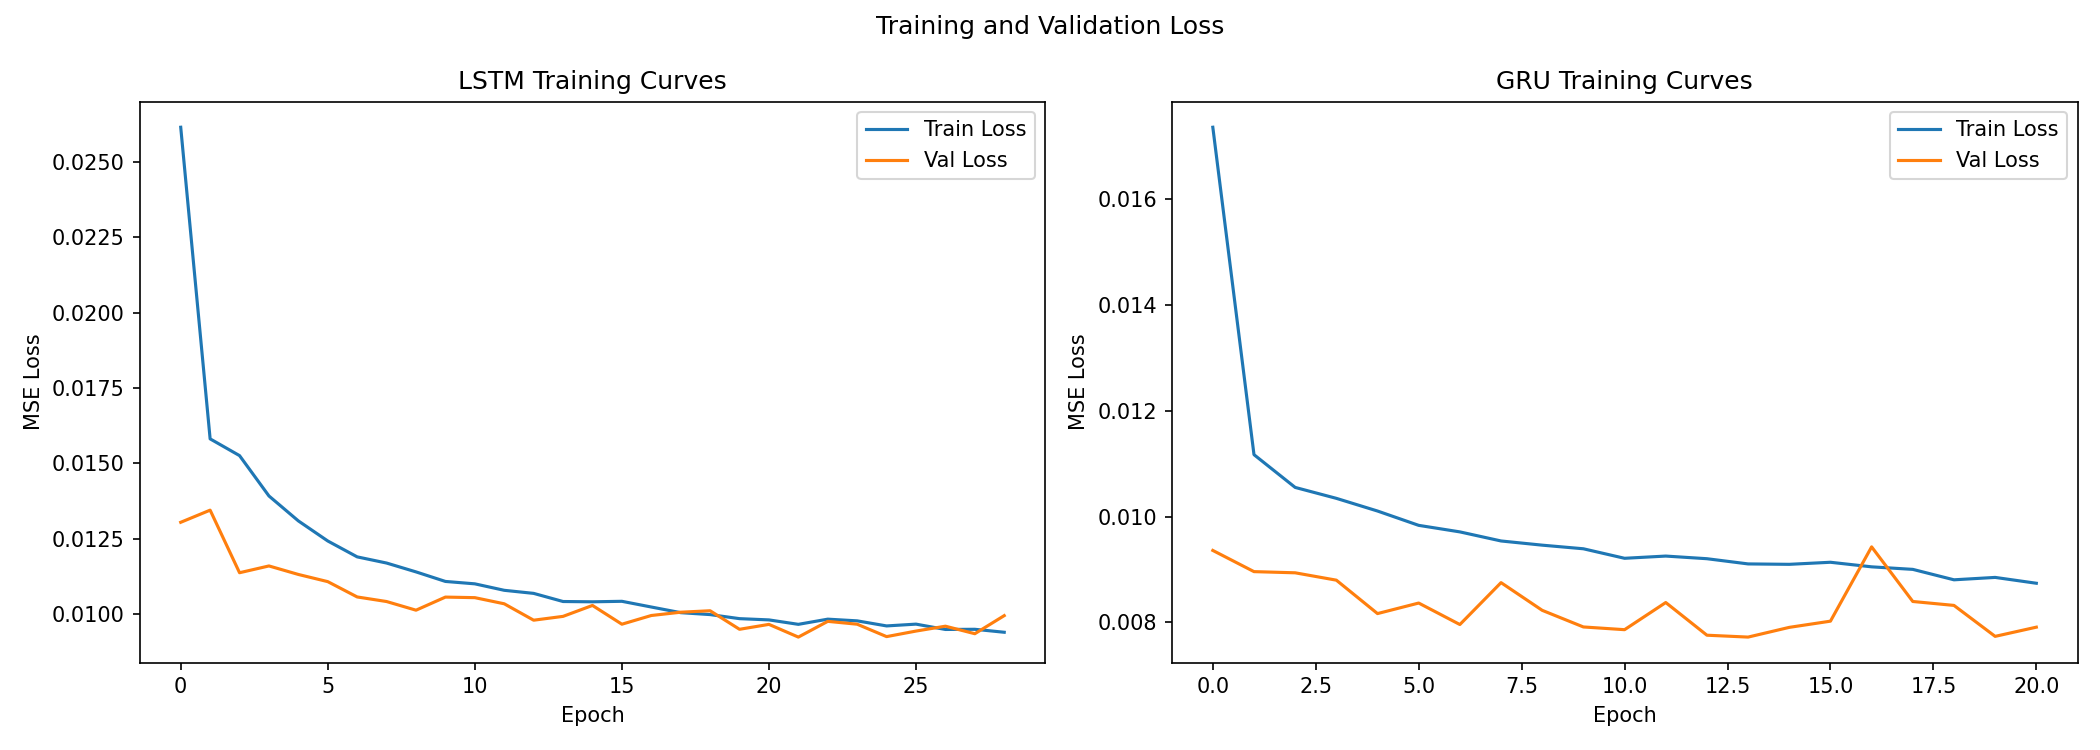
\includegraphics[width=\textwidth]{../results/training_curves.png}
\caption{Training and validation loss curves for the best LSTM (left) and GRU (right) configurations (Run 1). The GRU converges faster and shows a 
tighter train--validation gap, indicating less overfitting.}
\label{fig:training_curves}
\end{figure}

\begin{figure}[htbp]
\centering
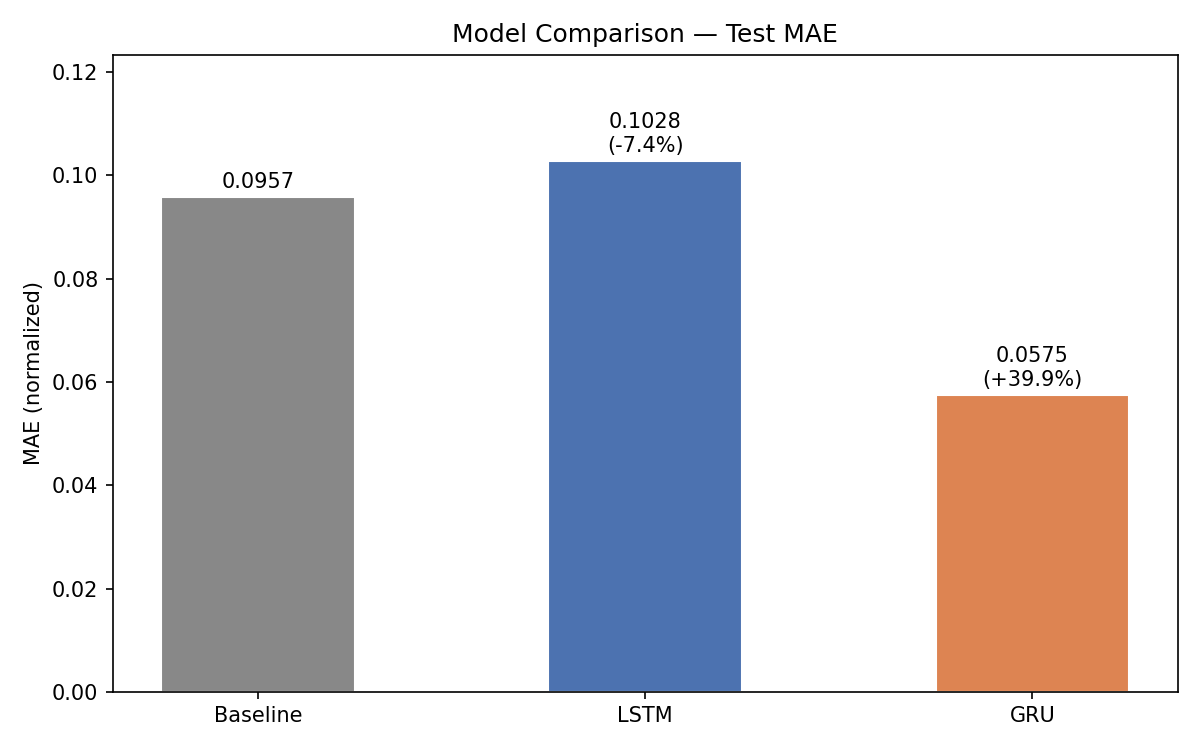
\includegraphics[width=0.65\textwidth]{../results/mae_comparison.png}
\caption{Test MAE for the baseline, best LSTM, and GRU on Run 1 (2023 data, 14k sequences). The GRU achieves a 39.9\% improvement over the moving 
average baseline; the default LSTM slightly underperforms it.}
\label{fig:mae_comparison}
\end{figure}

\subsubsection{Strategy Accuracy Progression}

Table~\ref{tab:strategy} traces strategy accuracy across all five phases of strategy-level development. The largest single jump is Phase 2 
(+26.2 percentage points), driven by splitting training by tire compound. Phase 3 and Phase 4 both regressed and were reverted; the final system
 uses the Phase 2 compound-specific configuration evaluated over 122 race-driver combinations.

\begin{table}[ht]
\centering
\caption{Strategy Accuracy Across All Phases}
\label{tab:strategy}
\begin{tabular}{lllr}
\toprule
Phase & Key Change & Evaluations & Accuracy \\
\midrule
Baseline (single-stop, shared GRU) & --- & 42 & 31.0\% \\
Phase 1: Multi-stop simulation & Brute-force 2-stop search & 42 & 35.7\% \\
Phase 2: Compound-specific GRUs & Separate model per compound & 42 & 61.9\% \\
Phase 3: Min first-pit constraint & Hard minimum lap threshold & 42 & 59.5\% (reverted) \\
Phase 4: Longer sequence (seq=15) & Window length 10$\to$15 laps & 42 & 50.0\% (reverted) \\
\textbf{Phase 5: 6-driver eval} & \textbf{Expanded to 122 evaluations} & \textbf{122} & \textbf{52.5\%} \\
\bottomrule
\end{tabular}
\end{table}

\subsubsection{Compound-Specific Model Results (Phase 2)}

Separate GRU models are trained on sequences filtered by the compound active at each timestep. Table~\ref{tab:compound} shows training results 
for the three compound-specific models. The HARD model benefits most from the compound split (14.1\% lower MAE than the mean-delta baseline), likely because hard-compound
stints are longer and the degradation signal is more gradual, giving a homogeneous training distribution the most leverage.

\begin{table}[ht]
\centering
\caption{Phase 2 Compound-Specific GRU Training Results}
\label{tab:compound}
\begin{tabular}{lrrr}
\toprule
Model & Train Sequences & Test MAE & vs.\ Mean-Delta Baseline \\
\midrule
gru\_delta\_soft   & 4,087  & 0.042113 & $-$10.2\% \\
gru\_delta\_medium & 9,853  & 0.037233 & $-$10.9\% \\
gru\_delta\_hard   & 15,041 & 0.035449 & $-$14.1\% \\
\bottomrule
\end{tabular}
\end{table}

\subsubsection{Per-Driver Accuracy}

Table~\ref{tab:drivers} shows strategy accuracy broken down by driver in the full 6-driver evaluation. The 30\% spread across drivers is the single most important finding for understanding system limitations.

\begin{table}[ht]
\centering
\caption{Per-Driver Strategy Accuracy (Phase 5, 122 evaluations)}
\label{tab:drivers}
\begin{tabular}{llrrrr}
\toprule
Driver & Team & Correct & Evaluated & Accuracy & Median Error (laps) \\
\midrule
RUS & Mercedes & 14 & 20 & \textbf{70.0\%} & 4.0 \\
SAI & Ferrari  & 12 & 20 & 60.0\% & 4.5 \\
VER & Red Bull & 11 & 21 & 52.4\% & 5.0 \\
NOR & McLaren  & 10 & 21 & 47.6\% & 11.0 \\
LEC & Ferrari  &  9 & 20 & 45.0\% & 7.0 \\
HAM & Mercedes &  8 & 20 & 40.0\% & 11.5 \\
\midrule
\textbf{Overall} & & \textbf{64} & \textbf{122} & \textbf{52.5\%} & \textbf{6.5} \\
\bottomrule
\end{tabular}
\end{table}

Figure~\ref{fig:strategy_examples} shows two representative strategy predictions that illustrate both ends of the accuracy spectrum. In the VER example (Round 1, Bahrain), the predicted pit window correctly brackets the actual pit stop at lap 38 and the cumulative delta chart confirms the crossover is clearly detected. In the NOR example (Round 3, Australia), the actual pit occurred on lap 13---an early undercut driven by track position---while the model predicted a window beginning around lap 35. This race represents the primary failure mode: reactive, non-degradation-driven pit stops that no lap time model can anticipate.

\begin{figure}[H]
\centering
\begin{subfigure}[t]{0.49\textwidth}
    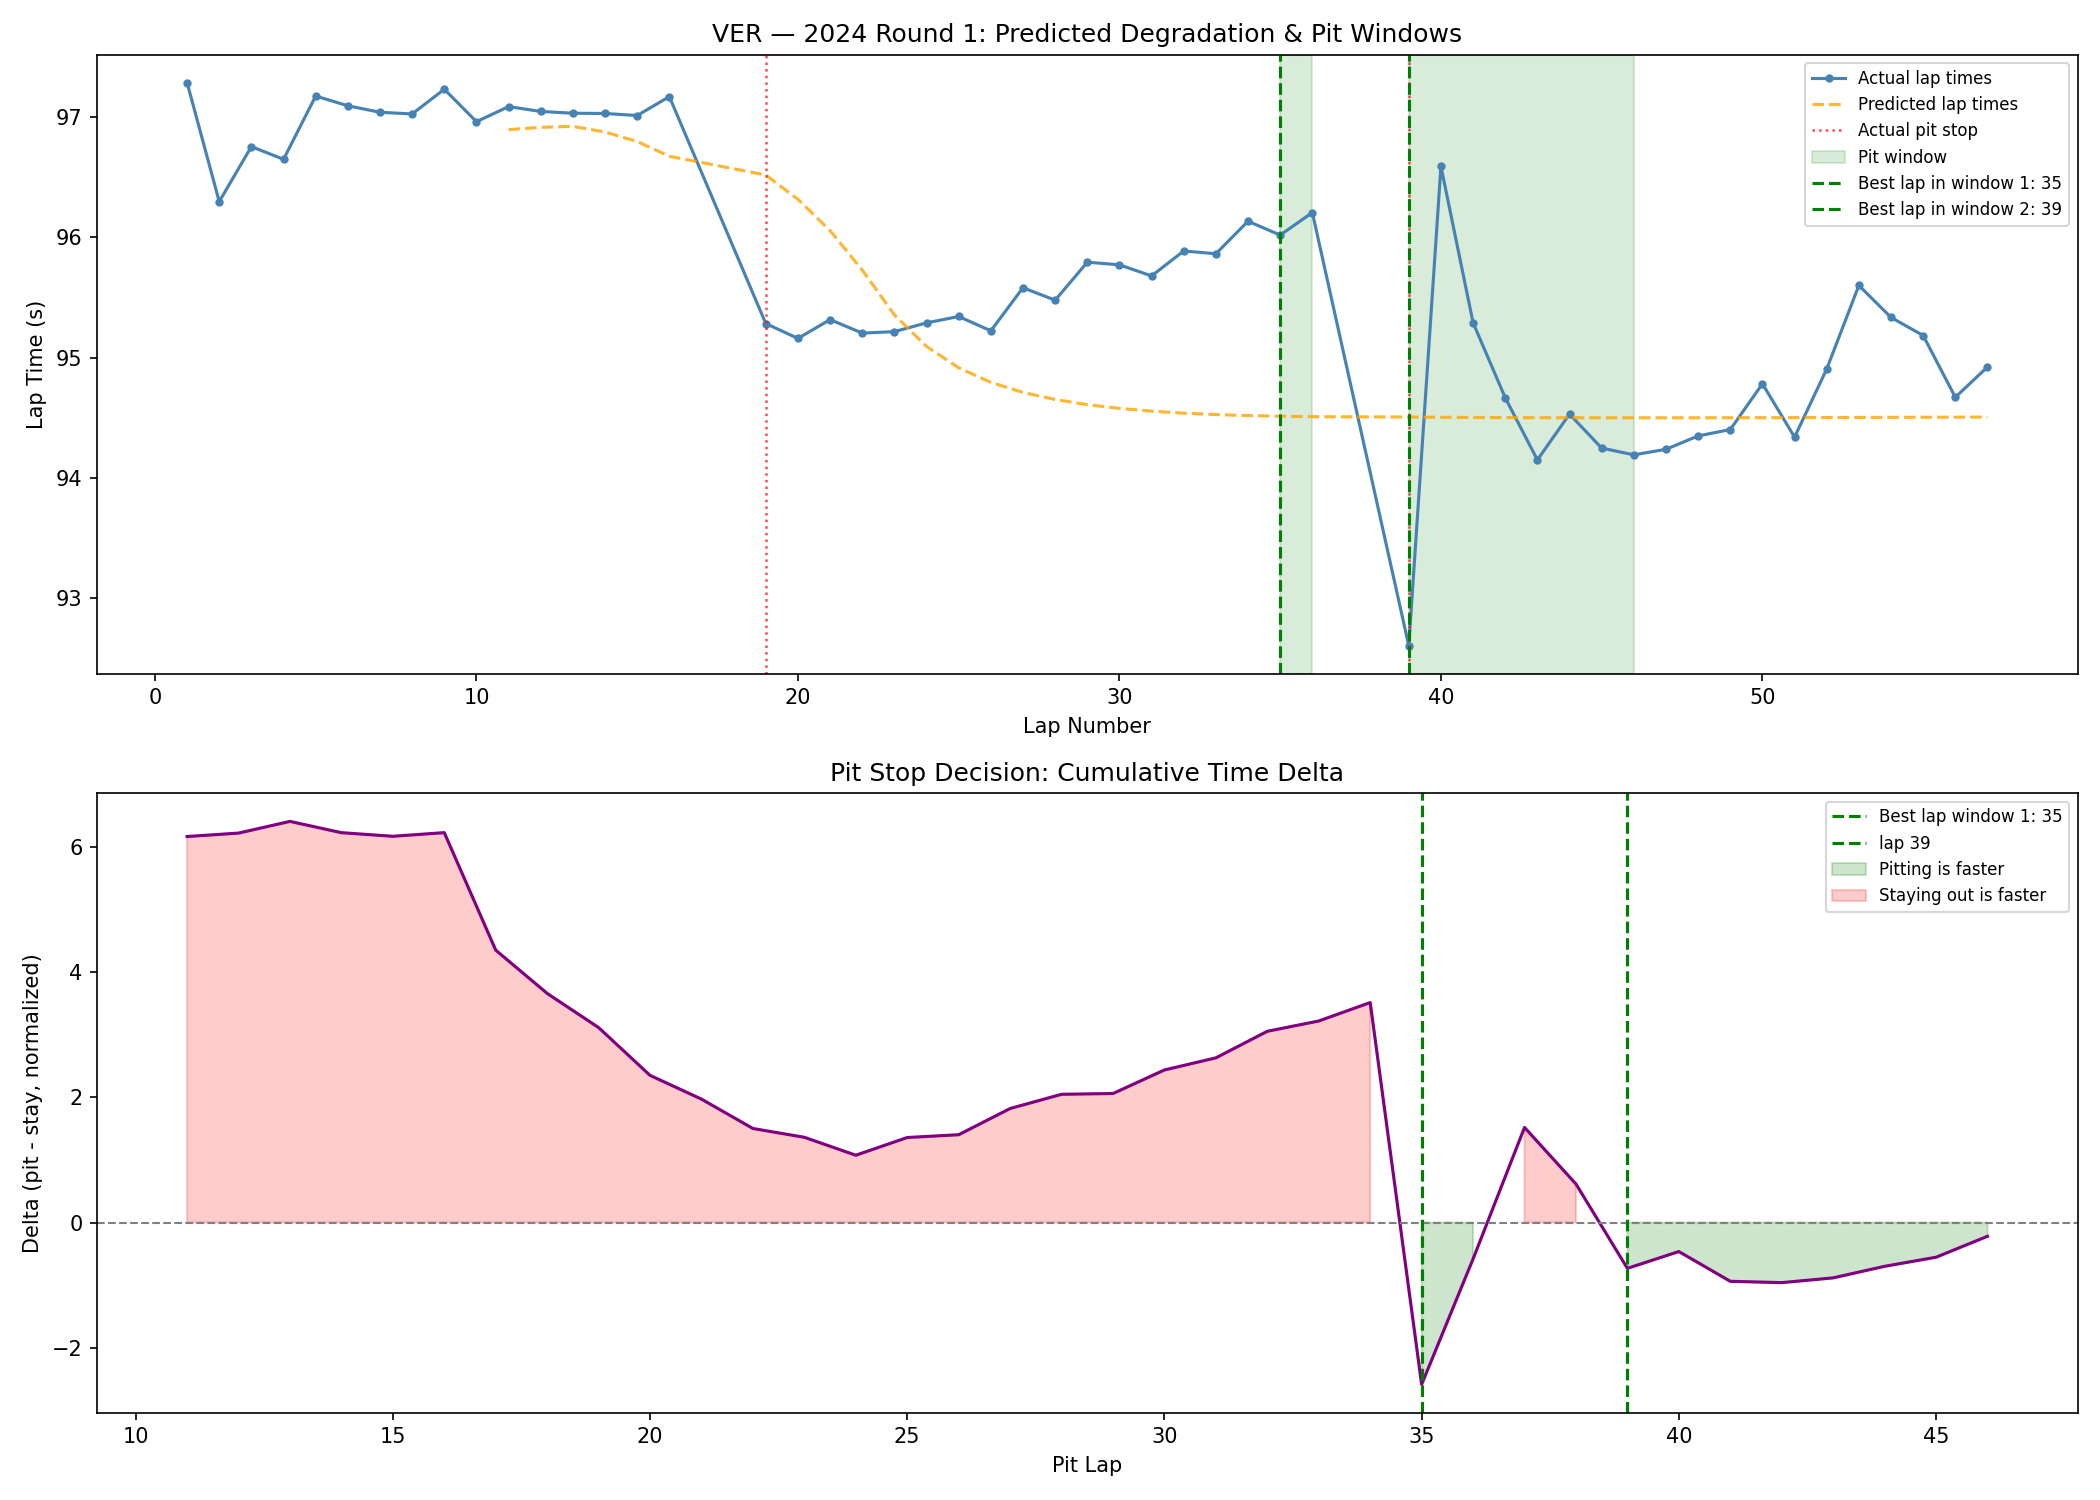
\includegraphics[width=\linewidth]{../results/strategy_VER_2024_r1.png}
    \caption{VER, Round 1 (Bahrain): correct prediction. Predicted pit window (green) brackets the actual stop at lap~38.}
    \label{fig:strat_ver}
\end{subfigure}
\hfill
\begin{subfigure}[t]{0.49\textwidth}
    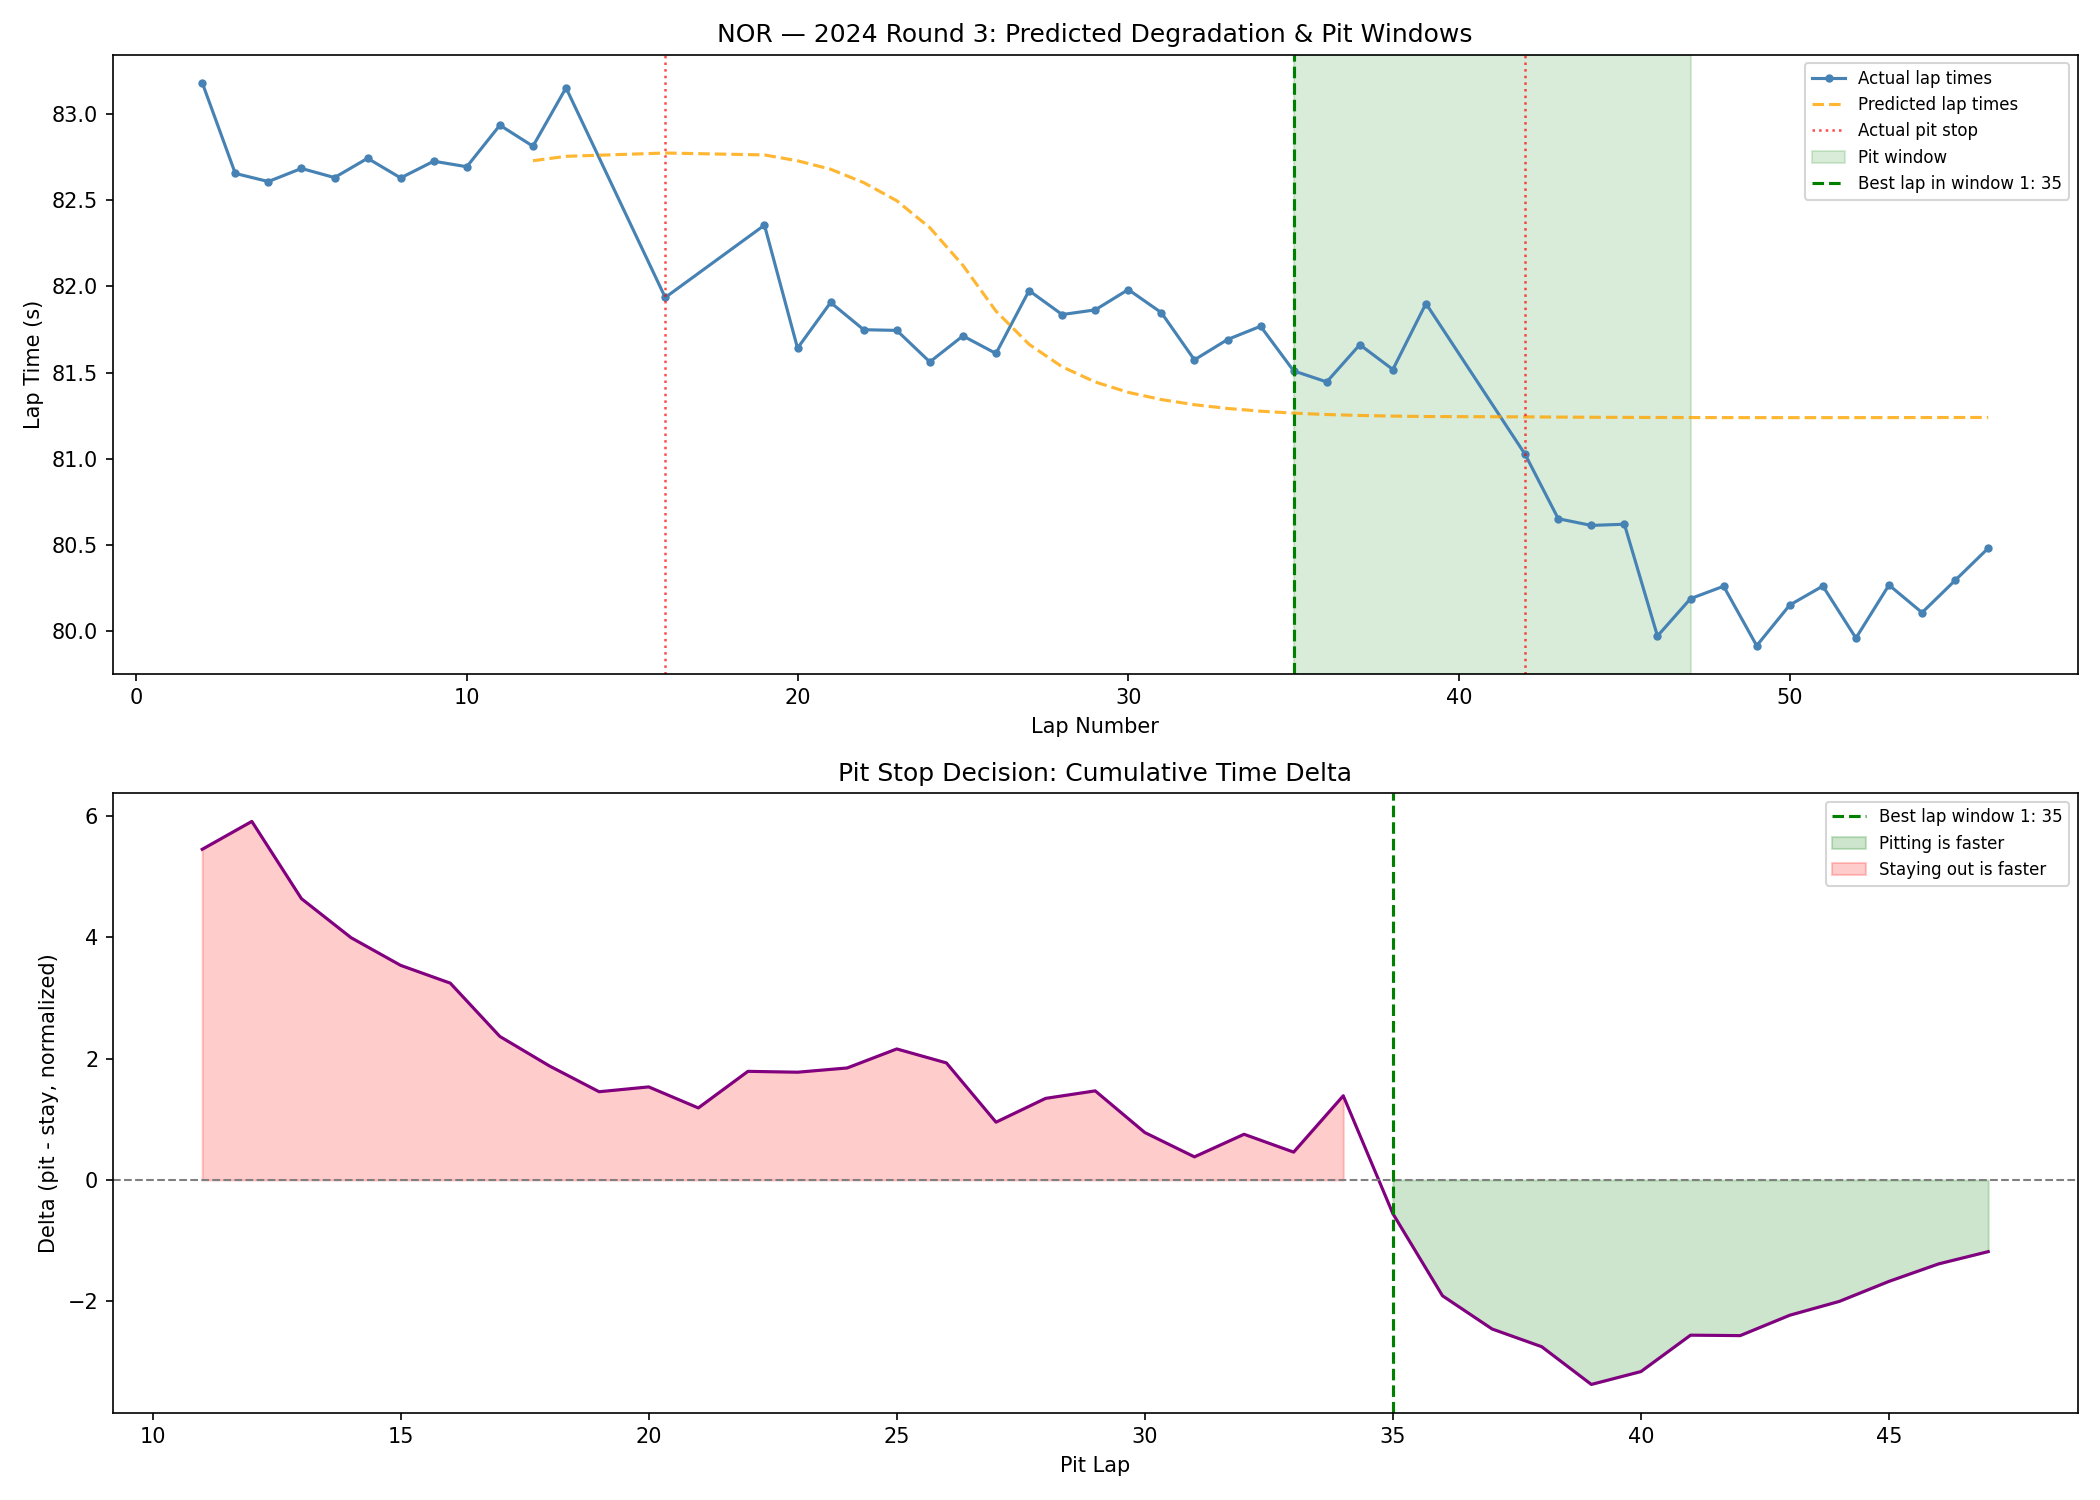
\includegraphics[width=\linewidth]{../results/strategy_NOR_2024_r3.png}
    \caption{NOR, Round 3 (Australia): miss. Actual stop on lap~13 was a tactical undercut; model predicted degradation-driven window at lap~35+.}
\label{fig:strat_nor}
\end{subfigure}
\caption{Representative strategy predictions. Top panel: actual vs.\ predicted lap times and predicted pit window. Bottom panel: cumulative time delta (positive = staying out is faster, negative = pitting is faster).}
\label{fig:strategy_examples}
\end{figure} 

\subsection{Analysis}\label{sec:analysis}

\subsubsection{GRU Dominates LSTM Variants}

The GRU outperformed all LSTM variants in every experimental configuration (Table~\ref{tab:architectures}, Figures~\ref{fig:training_curves}--\ref{fig:mae_comparison}). The margin is large: the GRU achieved a 38--40\% MAE improvement over the baseline, while the best-case LSTM only achieved 4--31\%.
Two factors explain this:

\textit{Parameter efficiency}: GRU has 39{,}425 parameters vs.\ 52{,}545 for LSTM (a 25\% reduction), lowering overfitting risk on a 28,000-sample training set. The consistent performance of high-dropout LSTM (+31.5\%) confirms that overfitting,not capacity, is the binding constraint.

\textit{Short sequence suitability}: With a 10-lap window, the cell state memory advantage of LSTM is irrelevant. Degradation within a 10-lap stint is approximately monotonic; complex long-range dependencies are absent. GRU's simpler update mechanism is well-matched to this structure.

\subsubsection{Attention Fails at Short Sequences}

LSTM with additive attention performed worst of all variants ($-22.5\%$ vs.\ baseline). With only 10 timesteps, the variation across hidden states is too small for the attention layer to learn a discriminative weighting; weights collapse toward uniform, and the additional non-linearity introduces noise. This is consistent with prior work showing attention benefits sequences of 20+ timesteps~\cite{bahdanau2015}.

\subsubsection{Delta Target is the Key Representation}

Switching the training target from absolute lap time to lap-to-lap delta ($\Delta t$) roughly doubled strategy accuracy (9.5\% $\to$ 19.0\%) on the original 42-evaluation pre-Phase-1 subset, without changing the model architecture. The 9.5\% baseline is the absolute-lap-time GRU result reported in Table~\ref{tab:decoupled} (Run 2 GRU); 19.0\% is the same architecture retrained on the delta target before any of the strategy-level phases in Table~\ref{tab:strategy} were applied. The improvement is conceptually clean since absolute lap time prediction forces the model to jointly explain baseline circuit pace and the marginal degradation signal, which are entangled in the normalized feature space. The delta formulation isolates the degradation rate as the sole target, which is what the strategy simulator actually needs.

Figure~\ref{fig:predictions} shows GRU predictions against held-out 2024 lap time sequences. The time series panel (top) shows the model tracking the degradation slope within each stint, including step changes at pit stops. The scatter plot (bottom) reveals a slight underprediction bias at high normalized lap times---corresponding to heavily degraded tires late in stints---which is where the pit crossover signal is most critical.

\begin{figure}[htbp]
\centering
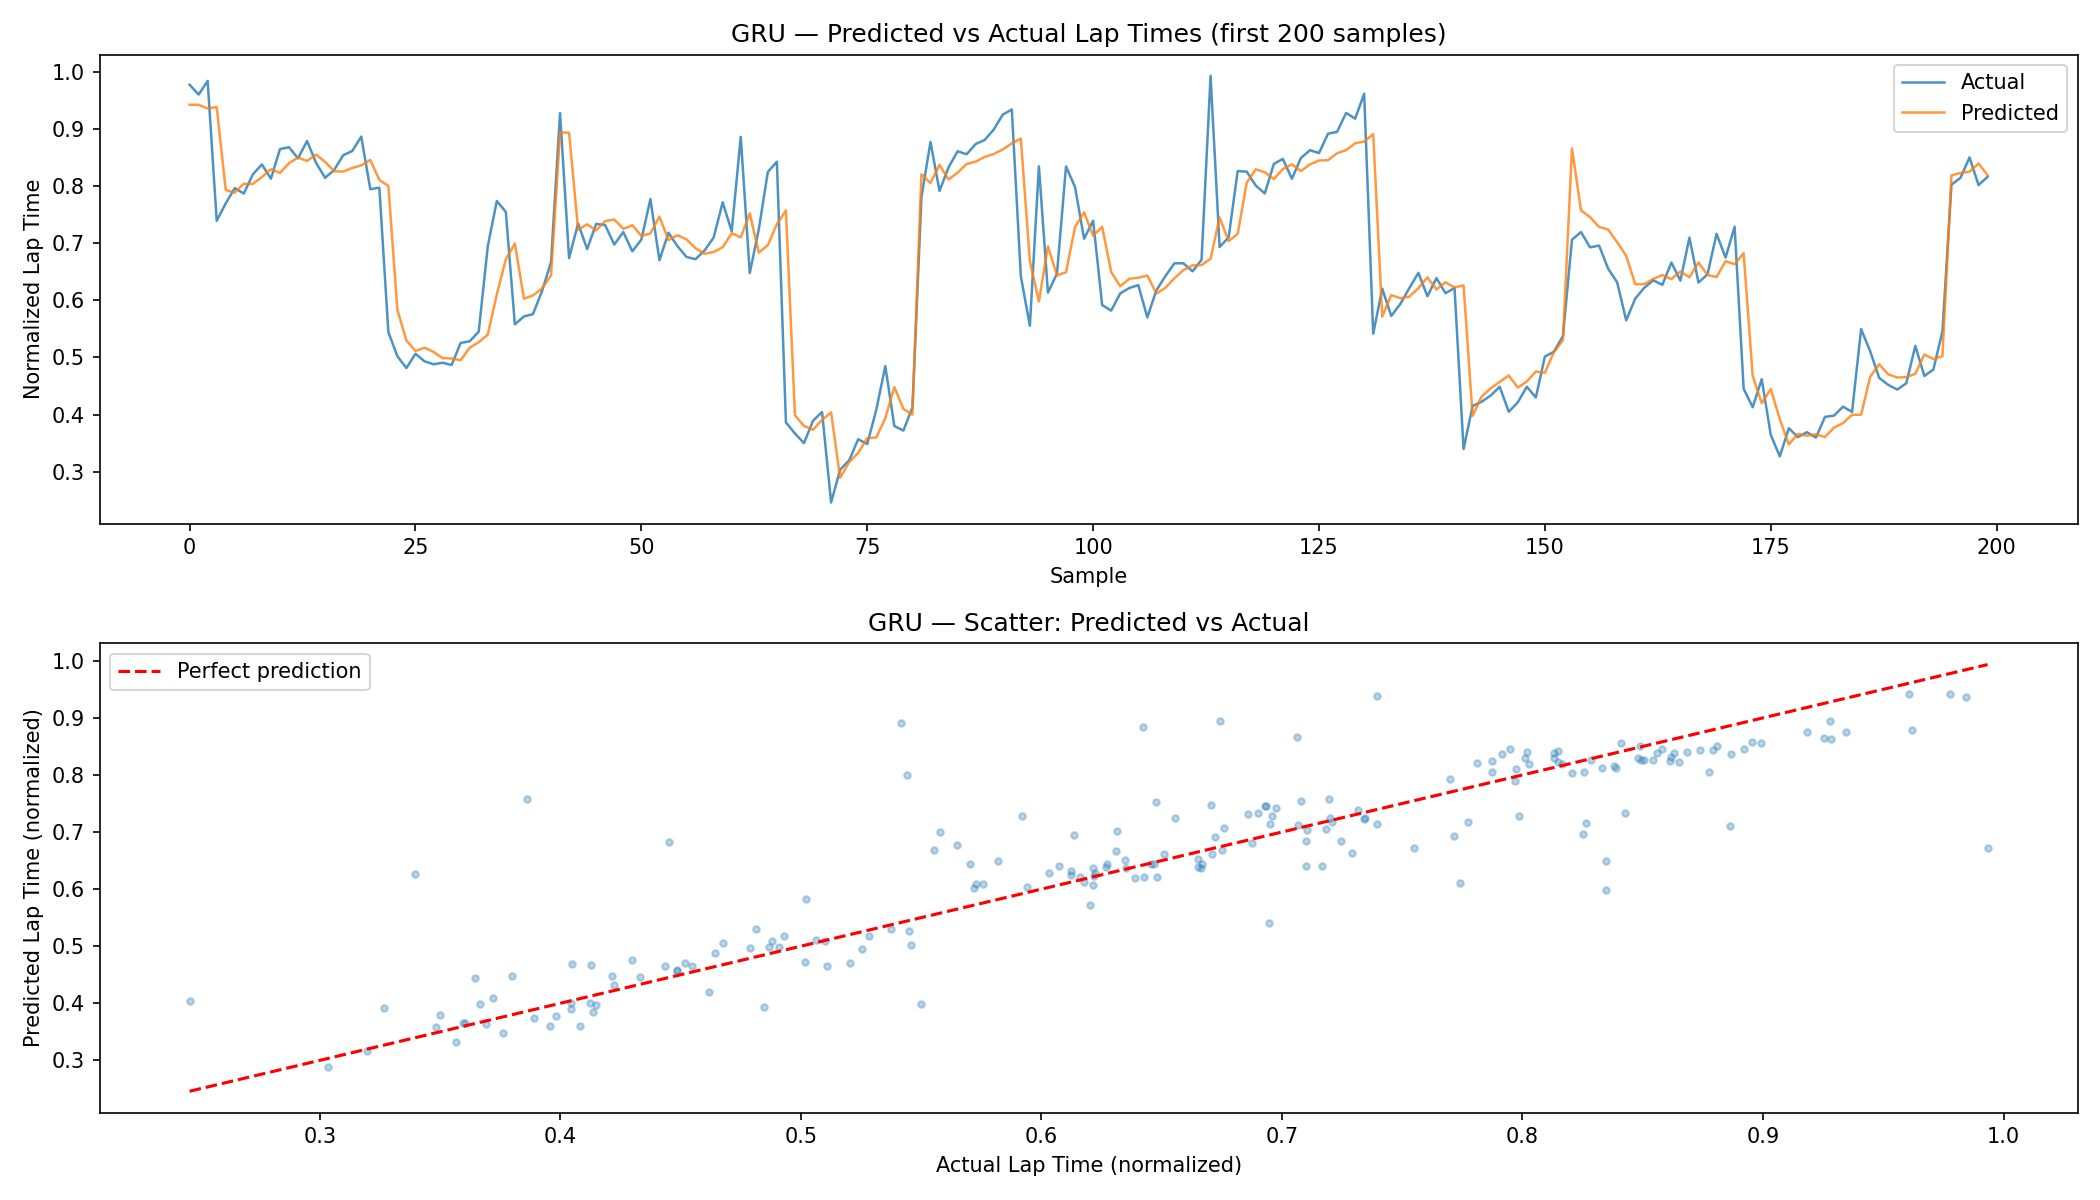
\includegraphics[width=\textwidth]{../results/predictions_gru.png}
\caption{GRU predictions on held-out 2024 sequences (first 200 samples). Top: predicted vs.\ actual lap time over time, showing accurate tracking of within-stint degradation slopes. Bottom: scatter of predicted vs.\ actual; the slight underprediction at high lap times indicates the model conservatively underestimates late-stint degradation.}
\label{fig:predictions}
\end{figure}

\FloatBarrier
\subsubsection{MAE and Strategy Accuracy Are Decoupled}

A striking pattern across three separate experiments is that lower test MAE does not imply higher strategy accuracy (Table~\ref{tab:decoupled}). Run 3 achieves the best MAE improvement (+40\%) but produces 0\% strategy accuracy. Run 6 (which adds the globally-normalized \texttt{TrackTemp\_global} feature alongside the existing per-race \texttt{TrackTemp}, giving the model both a circuit-relative and an absolute temperature signal) achieves better MAE than the best strategy-level configuration but yields only 2.4\% strategy accuracy.

\begin{table}[ht]
\centering
\caption{MAE vs.\ Strategy Accuracy Divergence}
\label{tab:decoupled}
\begin{tabular}{llrr}
\toprule
Configuration & Change & MAE Improvement & Strategy Accuracy \\
\midrule
Run 2 GRU & Baseline GRU & +38.5\% & 9.5\% \\
Run 3 GRU & SC filtering & +40.0\% & 0\% \\
Run 6 GRU & Global TrackTemp & +41.8\% & 2.4\% \\
Phase 2 compound GRU & Compound split & --- & \textbf{61.9\%} \\
\bottomrule
\end{tabular}
\end{table}

This divergence occurs because MAE measures accuracy on the test lap time distribution, while strategy accuracy measures timing quality on a different task: detecting the crossover point where pitting becomes net beneficial. A model that explains circuit-level temperature signals well (Run 6) may have lower MAE, but predict degradation slopes that are biased by those irrelevant signals, leading to systematically wrong pit timing.

\FloatBarrier
\subsubsection{Compound-Specific Models Are the Key Breakthrough}

The single largest accuracy improvement is achieved in Phase 2 by splitting training by tire compound ($+26.2$ percentage points over Phase 1). A shared GRU must average degradation behavior across SOFT, MEDIUM, and HARD compounds, whose degradation rates differ by a factor of 2--3. A compound-specific model sees only the degradation behavior relevant to the current tire, producing sharper predictions near the pit window crossover.

\FloatBarrier
\subsubsection{Negative Experiments}

Two experiments were reverted after causing regression:

\textit{Phase 3 --- Minimum first-pit constraint}: A hard lower bound of $\max(15, 0.2 \times L_\text{total})$ laps was imposed on the first pit recommendation to eliminate spurious early-pit predictions. This yielded 59.5\% (vs.\ 61.9\%), as it broke two races where early pits (laps 13--15) were strategically correct (Japan undercut, China sprint). A fixed minimum is too blunt without circuit-specific context.

\textit{Phase 4 --- Longer sequence (seq=15)}: Increasing the window from 10 to 15 laps reduced training sequences by 15\% (fewer stints long enough to yield 15-lap windows) and shifted the model's first-prediction opportunity later in each stint, producing an accuracy of 50.0\%.

\FloatBarrier
\subsubsection{Per-Driver Spread Reveals Identity Bottleneck}

The 30 percent spread in Table~\ref{tab:drivers} (HAM 40\% $\to$ RUS 70\%) cannot be explained by team effects---same-team pairs diverge significantly (HAM 40\% vs.\ RUS 70\% on Mercedes; LEC 45\% vs.\ SAI 60\% on Ferrari). This points to driver-specific stint patterns that the current model cannot capture. Russell ran notably more conservative stint strategies in 2024 (later first pits, consistent MEDIUM stints) that align well with the model's predictions; Hamilton's more aggressive tire management and frequent off-sequence stops are harder to predict.

The NOR miss in Figure~\ref{fig:strat_nor} is emblematic of this class of failure. The model correctly identifies when degradation would warrant a stop, but cannot anticipate that the team will sacrifice lap time to execute a tactical undercut instead. The model has no driver or team identity feature. Adding driver one-hot encoding or team-level embeddings would be the most impactful next step.

\section{Conclusions}

\subsection{Summary}

This project demonstrates that publicly available F1 lap time data, combined with compound-specific GRU sequence models and a simulation-based strategy evaluator, can recommend pit stop windows with 52.5\% accuracy across 122 race-driver evaluations from the 2024 season. The result represents a +21.5 percentage-point improvement over a brute-force multi-stop baseline. The GRU architecture with delta target, compound-specific training, and per-race normalization is the configuration that best captures the tire degradation signal relevant to strategy timing.

The project does not meet the $\geq$70\% secondary accuracy criterion set at the outset, though one driver (Russell) reaches exactly 70\% in isolation. The 61.9\% result on the original 2-driver subset (Verstappen and Norris) is the strongest single-configuration result but is best understood as an upper bound on favorable conditions; 52.5\% on 122 evaluations is the honest large-sample estimate.

\subsection{Contributions}

This project makes the following contributions:

\begin{itemize}[noitemsep]
    \item A full open-source pipeline for F1 pit stop strategy evaluation using only publicly available data (FastF1 API, 2022--2024 seasons).
    \item An empirical demonstration that compound-specific sequence modeling dramatically outperforms shared-compound models for strategy timing ($+26.2$ pp).
    \item A systematic ablation showing that MAE on lap time prediction is a poor proxy for strategy accuracy, with three experiments showing conflicting directions.
    \item Quantification of the driver identity gap: per-driver accuracy ranges from 40\% to 70\% in the same evaluation, setting a clear target for future work.
    \item Documentation of five strategy-level experimental phases including two fully reverted experiments with root-cause analysis.
\end{itemize}

\subsection{Future Work}

The most impactful near-term improvement is adding driver and team identity features. Even a simple driver one-hot encoding over the 20 F1 drivers would allow the model to learn driver-specific degradation tendencies and strategy preferences. Based on the Phase 5 analysis, this feature alone could close a substantial portion of the per-driver accuracy gap.

Additional directions include:
\begin{itemize}[noitemsep]
    \item \textbf{More training data}: Adding 2021 and 2020 season data would triple the training set. The LSTM deep ablation showed that deeper models directly benefit from more data.
    \item \textbf{Track identity features}: Circuit-specific embeddings would allow the model to learn that Monaco and Singapore have different degradation profiles than Bahrain and Spa.
    \item \textbf{Competitor position}: Real teams pit partly based on gap to the driver ahead or behind. Including relative position would move the system closer to true strategy modeling.
    \item \textbf{Transformer architecture}: With driver/track identity tokens, a transformer encoder \cite{vaswani2017} over the 10-lap sequence may outperform the GRU, as cross-stint attention becomes meaningful once distinct sequence types are identifiable.
\end{itemize}

\begin{thebibliography}{99}

\bibitem{fastf1}
T.\ Pretzel, ``FastF1: A Python package for accessing Formula 1 data,'' GitHub repository, 2024. [Online]. Available: \url{https://github.com/theOehrly/Fast-F1}

\bibitem{hochreiter1997}
S.\ Hochreiter and J.\ Schmidhuber, ``Long short-term memory,'' \textit{Neural Computation}, vol.\ 9, no.\ 8, pp.\ 1735--1780, 1997.

\bibitem{cho2014}
K.\ Cho, B.\ van Merrienboer, C.\ Gulcehre, D.\ Bahdanau, F.\ Bougares, H.\ Schwenk, and Y.\ Bengio, ``Learning phrase representations using RNN encoder-decoder for statistical machine translation,'' in \textit{Proc.\ EMNLP}, 2014, pp.\ 1724--1734.

\bibitem{chung2014}
J.\ Chung, C.\ Gulcehre, K.\ Cho, and Y.\ Bengio, ``Empirical evaluation of gated recurrent neural networks on sequence modeling,'' in \textit{NIPS Workshop on Deep Learning}, 2014.

\bibitem{bahdanau2015}
D.\ Bahdanau, K.\ Cho, and Y.\ Bengio, ``Neural machine translation by jointly learning to align and translate,'' in \textit{Proc.\ ICLR}, 2015.

\bibitem{kingma2015}
D.\ P.\ Kingma and J.\ Ba, ``Adam: A method for stochastic optimization,'' in \textit{Proc.\ ICLR}, 2015.

\bibitem{heilmeier2020}
A.\ Heilmeier, M.\ Thomaser, M.\ Graf, and J.\ Betz, ``A race simulation for strategy decisions in circuit motorsports,'' in \textit{Proc.\ IEEE 23rd International Conference on Intelligent Transportation Systems (ITSC)}, 2020, pp.\ 1--8.

\bibitem{tulabandhula2014}
T.\ Tulabandhula and C.\ Rudin, ``On combining machine learning with decision making,'' \textit{Machine Learning}, vol.\ 97, no.\ 1, pp.\ 33--64, 2014.

\bibitem{vaswani2017}
A.\ Vaswani, N.\ Shazeer, N.\ Parmar, J.\ Uszkoreit, L.\ Jones, A.\ N.\ Gomez, L.\ Kaiser, and I.\ Polosukhin, ``Attention is all you need,'' in \textit{Proc.\ NeurIPS}, 2017.

\end{thebibliography}

\appendix
\section{Experiment Reproducibility}

All code is organized as follows:

\begin{itemize}[noitemsep]
    \item \texttt{data/pipeline.py}: FastF1 data fetching and feature engineering
    \item \texttt{data/preprocessing.py}: Sequence building, normalization, compound splitting
    \item \texttt{train.py}: Model training for all configurations
    \item \texttt{strategy/pit\_optimizer.py}: Strategy simulation and evaluation
    \item \texttt{models/}: LSTM, GRU, and attention model definitions
    \item \texttt{results/}: Saved model weights and evaluation CSVs
\end{itemize}

To reproduce the Phase 5 results from scratch:
\begin{enumerate}[noitemsep]
    \item \texttt{python data/preprocessing.py} --- regenerates training and test tensors
    \item \texttt{python train.py} --- trains the three compound-specific GRU models
    \item \texttt{PYTHONPATH=. python strategy/pit\_optimizer.py} --- runs strategy evaluation on all 6 drivers across the 2024 season
\end{enumerate}

Training requires approximately 10 minutes on Apple M-series hardware (MPS backend). The strategy evaluation requires approximately 40--60 minutes due to FastF1 data loading per race.


\end{document}
